\documentclass[a4paper,11pt]{article}

\usepackage{luatexja}
\usepackage{luatexja-fontspec}
\setmainjfont{Noto Serif CJK JP}
\setsansjfont{Noto Sans CJK JP}
\setmonojfont{Noto Sans Mono CJK JP}
\usepackage[margin=22mm]{geometry}
\usepackage{amsmath}
\usepackage{booktabs}
\usepackage{array}
\usepackage{enumitem}
\usepackage{graphicx}
\usepackage{xcolor}
\usepackage[hidelinks,unicode]{hyperref}
\emergencystretch=2em

\hypersetup{
  pdftitle={AJP MOBOにおけるCFD失敗点の原因診断},
  pdfauthor={AJP simulation workspace}
}

\title{AJP MOBOにおけるCFD失敗点の原因診断}
\author{AJP simulation workspace}
\date{2026年7月27日}

\begin{document}
\maketitle

\section{結論}

現行キャンペーンでCFD失敗点が落ちる直接原因は、メッシュ生成失敗でも
\texttt{kOmegaSST} のゼロ除算そのものでもなく、
\texttt{base/system/fvSolution} における圧力$p$の緩和指定である。
修正前は
\[
  \texttt{relaxationFactors/equations/p = 0.3}
\]
として圧力方程式をequation under-relaxationしていた。急な収縮形状では
圧力・速度連成が不安定となり、連続の式誤差が先に増大する。その後、
速度、圧力、乱流量がオーバーフローし、GAMGまたは乱流モデル内部で
浮動小数点例外（SIGFPE）になる。

圧力を
\[
  \boxed{\texttt{relaxationFactors/fields/p = 0.3}}
\]
へ移し、圧力場の更新量をfield under-relaxationするだけで、
同一形状、同一メッシュ、同一境界条件の3失敗ケースが800反復を
正常完走した。したがって、高い \texttt{theta0\_deg} は旧設定の
数値不安定性を顕在化させる条件であって、それだけを根拠に物理的な
不可能形状として除外すべきではない。

\section{解析対象}

目的関数バージョン
\texttt{central\_target\_d10um\_mobo\_v1}、
提案法 \texttt{qlognehvi} のうち、正常完了またはCFD失敗として
確定した179ケースを調べた。

\begin{center}
\begin{tabular}{lr}
\toprule
分類 & ケース数 \\
\midrule
正常完了 & 144 \\
CFD失敗 & 35 \\
\quad \texttt{simpleFoam} SIGFPE & 18 \\
\quad 乱流モデルdivideでSIGFPE & 1 \\
\quad \texttt{End}到達後に異常速度で棄却 & 13 \\
\quad 回収ログ上の未分類CFD失敗 & 3 \\
\bottomrule
\end{tabular}
\end{center}

失敗はXEON1、XEON4、XEON5、XEON6の全ホストで発生した。ホスト別
失敗率は15.0--27.1\%であり、単一サーバーのOpenFOAM環境または
ハードウェア故障では説明できない。

\section{ログから分かる故障順序}

35失敗ケースのすべてで、SIGFPEまたは終了時速度検査より前に
連続の式誤差が増大した。最初に誤差が$10^3$を超える反復は
113--980であり、その後$10^{12}$から最大$10^{131}$まで増加した。
故障順序は次の通りである。

\begin{enumerate}[leftmargin=24pt]
  \item 圧力・速度補正が不安定化する。
  \item continuity errorが反復ごとに増大する。
  \item $U$、$p$、$k$、$\omega$が非物理的な桁へ成長する。
  \item 圧力GAMGの内積、または乱流モデルの除算でSIGFPEになる。
  \item SIGFPEにならない場合も \texttt{End} まで異常場を計算し続け、
    最終的に \texttt{max(mag(U))} 検査で棄却される。
\end{enumerate}

したがって、スタックトレース末尾の乱流モデルdivideは最終的な
クラッシュ位置であり、発散の開始原因ではない。

\section{除外した原因}

\subsection{実行ホスト}

失敗は全4ホストへ分散しているため、XEON固有の故障ではない。

\subsection{メッシュ品質の単純な閾値}

成功2ケースと失敗2ケースを同じ
\texttt{checkMesh -allGeometry -allTopology} で比較した。

\begin{center}
\small
\begin{tabular}{lrrrrrl}
\toprule
ケース & 結果 & cells & max non-orth. & max skew. &
min det. & det.$<0.001$ \\
\midrule
\texttt{case\_1376} & 成功 & 15,439 & 59.16 & 1.581 &
$3.31{\times}10^{-4}$ & 6 \\
\texttt{case\_1380} & 成功 & 20,589 & 56.19 & 1.150 &
0 & 11 \\
\texttt{case\_1383} & 失敗 & 59,569 & 56.65 & 1.498 &
$3.30{\times}10^{-4}$ & 6 \\
\texttt{case\_1428} & 失敗 & 31,665 & 57.76 & 1.548 &
$3.27{\times}10^{-4}$ & 6 \\
\bottomrule
\end{tabular}
\end{center}

成功ケースにも同等以上のdeterminant警告があり、非直交性とskewnessも
失敗ケースだけが悪いわけではない。この警告は別途改善すべきだが、
今回の成否を識別しない。

\subsection{\texttt{potentialFoam}}

179ケースすべてで \texttt{potentialFoam} はSIGFPEとなったが、
144ケースはその後の \texttt{simpleFoam} を正常完了した。
当時の\texttt{base/run.sh}はこの失敗を意図的に無視していた。
したがって \texttt{potentialFoam} 失敗は現行フローの独立した不具合で
あり、35ケースだけが落ちる理由ではない。ただし、初期流れ場が生成
されず、\texttt{simpleFoam} が静止場から立ち上がるため、数値設定への
感度を高めている。

\paragraph{2026年9月8日の解決追記}
この不具合は、流量入口境界条件を評価しないまま
\texttt{potentialFoam}の\texttt{-writep}を実行し、全域$U=0$の状態で圧力近似の
流向filterを計算したことによる0除算であった。現行templateは
\texttt{potentialFoam -initialiseUBCs -writep}へ変更した。structured実meshの
local testでPhiと$p$が非ゼロ反復により収束し、SIGFPEなしで\texttt{End}へ
到達すること、および後続\texttt{simpleFoam}が正常に進むことを確認した。
失敗を無視する処理も廃止し、今後はpotential初期化失敗を
\texttt{CFD\_FAILED}として停止する。

\section{失敗しやすい形状領域}

\begin{figure}[htbp]
  \centering
  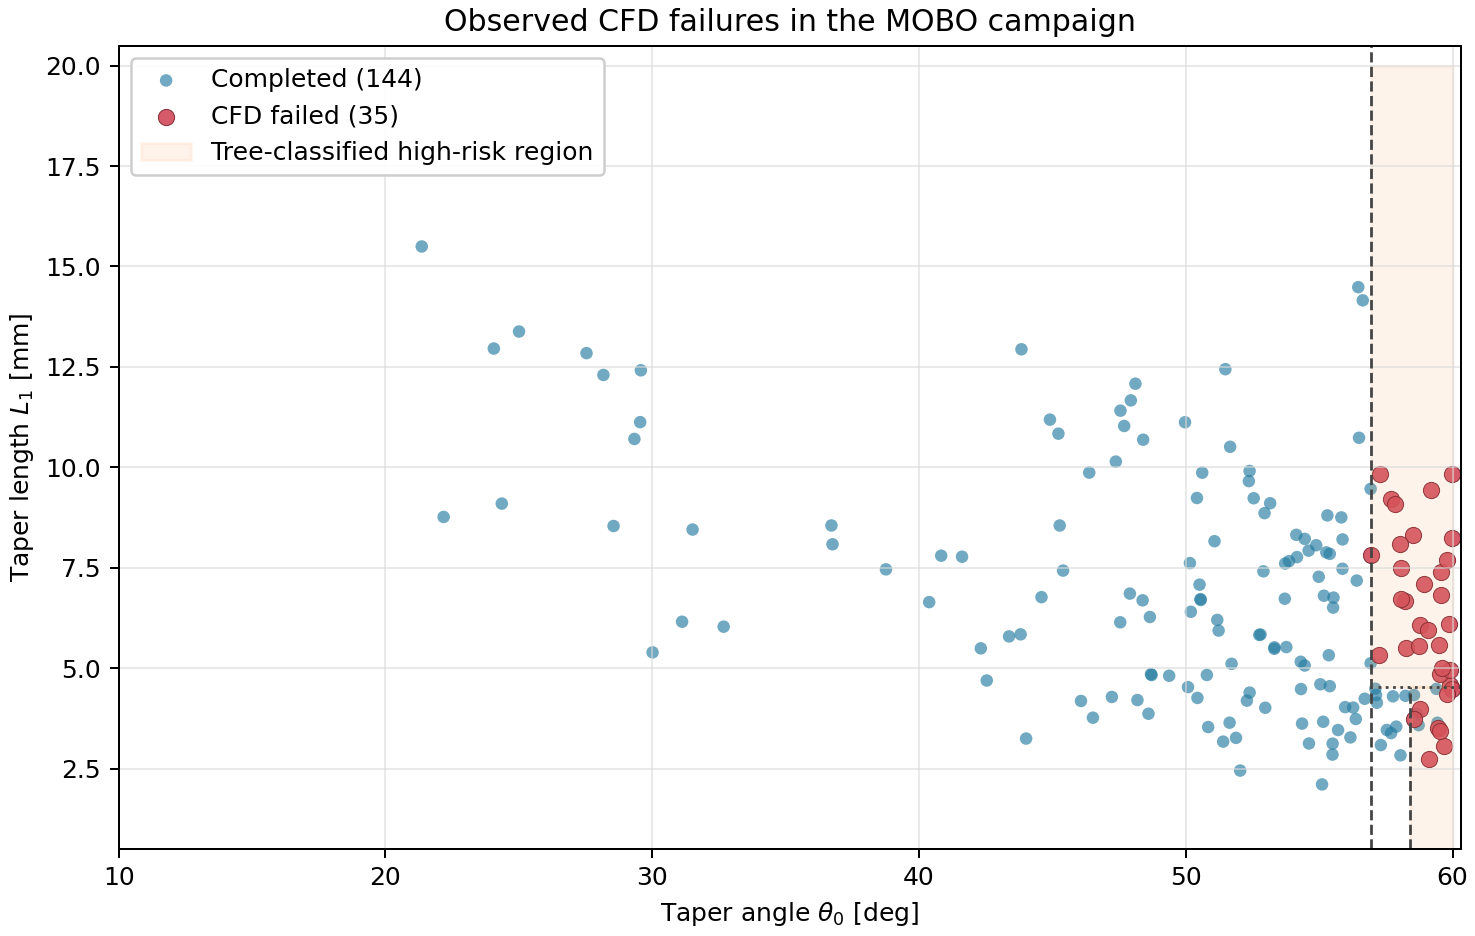
\includegraphics[width=\linewidth]{cfd_failure_map_20260727.png}
  \caption{179ケースにおける \texttt{theta0\_deg}、\texttt{L1\_mm} と
  CFD成否。着色部は浅い決定木が識別した高リスク領域である。}
\end{figure}

\texttt{theta0\_deg} の四分位別失敗率は次の通りであった。
\[
\begin{array}{c|c|c}
\text{範囲 [deg]} & \text{失敗数/総数} & \text{失敗率}\\
\hline
21.36\text{--}48.19 & 0/44 & 0\%\\
48.38\text{--}53.77 & 0/45 & 0\%\\
53.87\text{--}57.25 & 2/45 & 4.4\%\\
57.28\text{--}60.00 & 33/45 & 73.3\%
\end{array}
\]

深さ3の決定木は、交差検証balanced accuracy 0.944で
\[
\begin{aligned}
 \theta_0 &>56.9345^\circ,\quad L_1>4.5373~\mathrm{mm},\\
 \text{または}\quad
 \theta_0 &>58.3839^\circ,\quad L_1\leq4.5373~\mathrm{mm}
\end{aligned}
\]
を主な高リスク領域として識別した。特に第1条件内は観測27点中27点が
失敗した。ただし、これは旧数値設定に対する経験的な発生領域である。

\section{同一メッシュA/B試験}

\subsection{試験条件}

\texttt{case\_1317} を中心に、メッシュ、境界条件、離散化スキームを
固定し、\texttt{fvSolution} のみ変更した。

\begin{center}
\small
\begin{tabular}{
  >{\raggedright\arraybackslash}p{37mm}
  >{\raggedright\arraybackslash}p{55mm}
  >{\raggedright\arraybackslash}p{55mm}
}
\toprule
設定 & 変更 & 結果 \\
\midrule
元設定 &
\texttt{consistent yes}、
\texttt{equations/p=0.3} &
反復800でcontinuity $4.57{\times}10^5$、
最終最大速度$3.08{\times}10^7$ m/s \\
乱流無効 &
元の圧力緩和を維持しlaminar化 &
continuityは低下せず増加傾向。乱流を切っても解消しない \\
\texttt{consistent}のみno &
\texttt{equations/p=0.3}を維持 &
反復25でSIGFPE \\
SIMPLEC、圧力緩和なし &
\texttt{p}を緩和指定から除外 &
反復201でcontinuity 163まで増加したため停止 \\
SIMPLEC、field圧力緩和 &
\texttt{fields/p=0.3} &
反復800完走、continuity $7.87{\times}10^{-3}$、
最大速度51.58 m/s \\
標準SIMPLE、field圧力緩和 &
\texttt{consistent no}、
\texttt{fields/p=0.3} &
反復800完走、continuity $2.54{\times}10^{-3}$、
最大速度51.59 m/s \\
低緩和SIMPLE &
\texttt{fields/p=0.2}、
\texttt{U,k,\omega=0.3} &
反復800完走、continuity $1.34{\times}10^{-3}$、
最大速度53.31 m/s \\
\bottomrule
\end{tabular}
\end{center}

圧力を \texttt{fields} へ移した2方式がともに安定し、
\texttt{consistent} だけの切替では安定しなかった。したがって、
決定因子はSIMPLE/SIMPLECの選択そのものではなく、圧力緩和の種類である。
OpenFOAM公式文書もfield under-relaxationとequation
under-relaxationを別方式として定義している%
\footnote{\url{https://www.openfoam.com/documentation/user-guide/6-solving/6.3-solution-and-algorithm-control}}。

\begin{figure}[htbp]
  \centering
  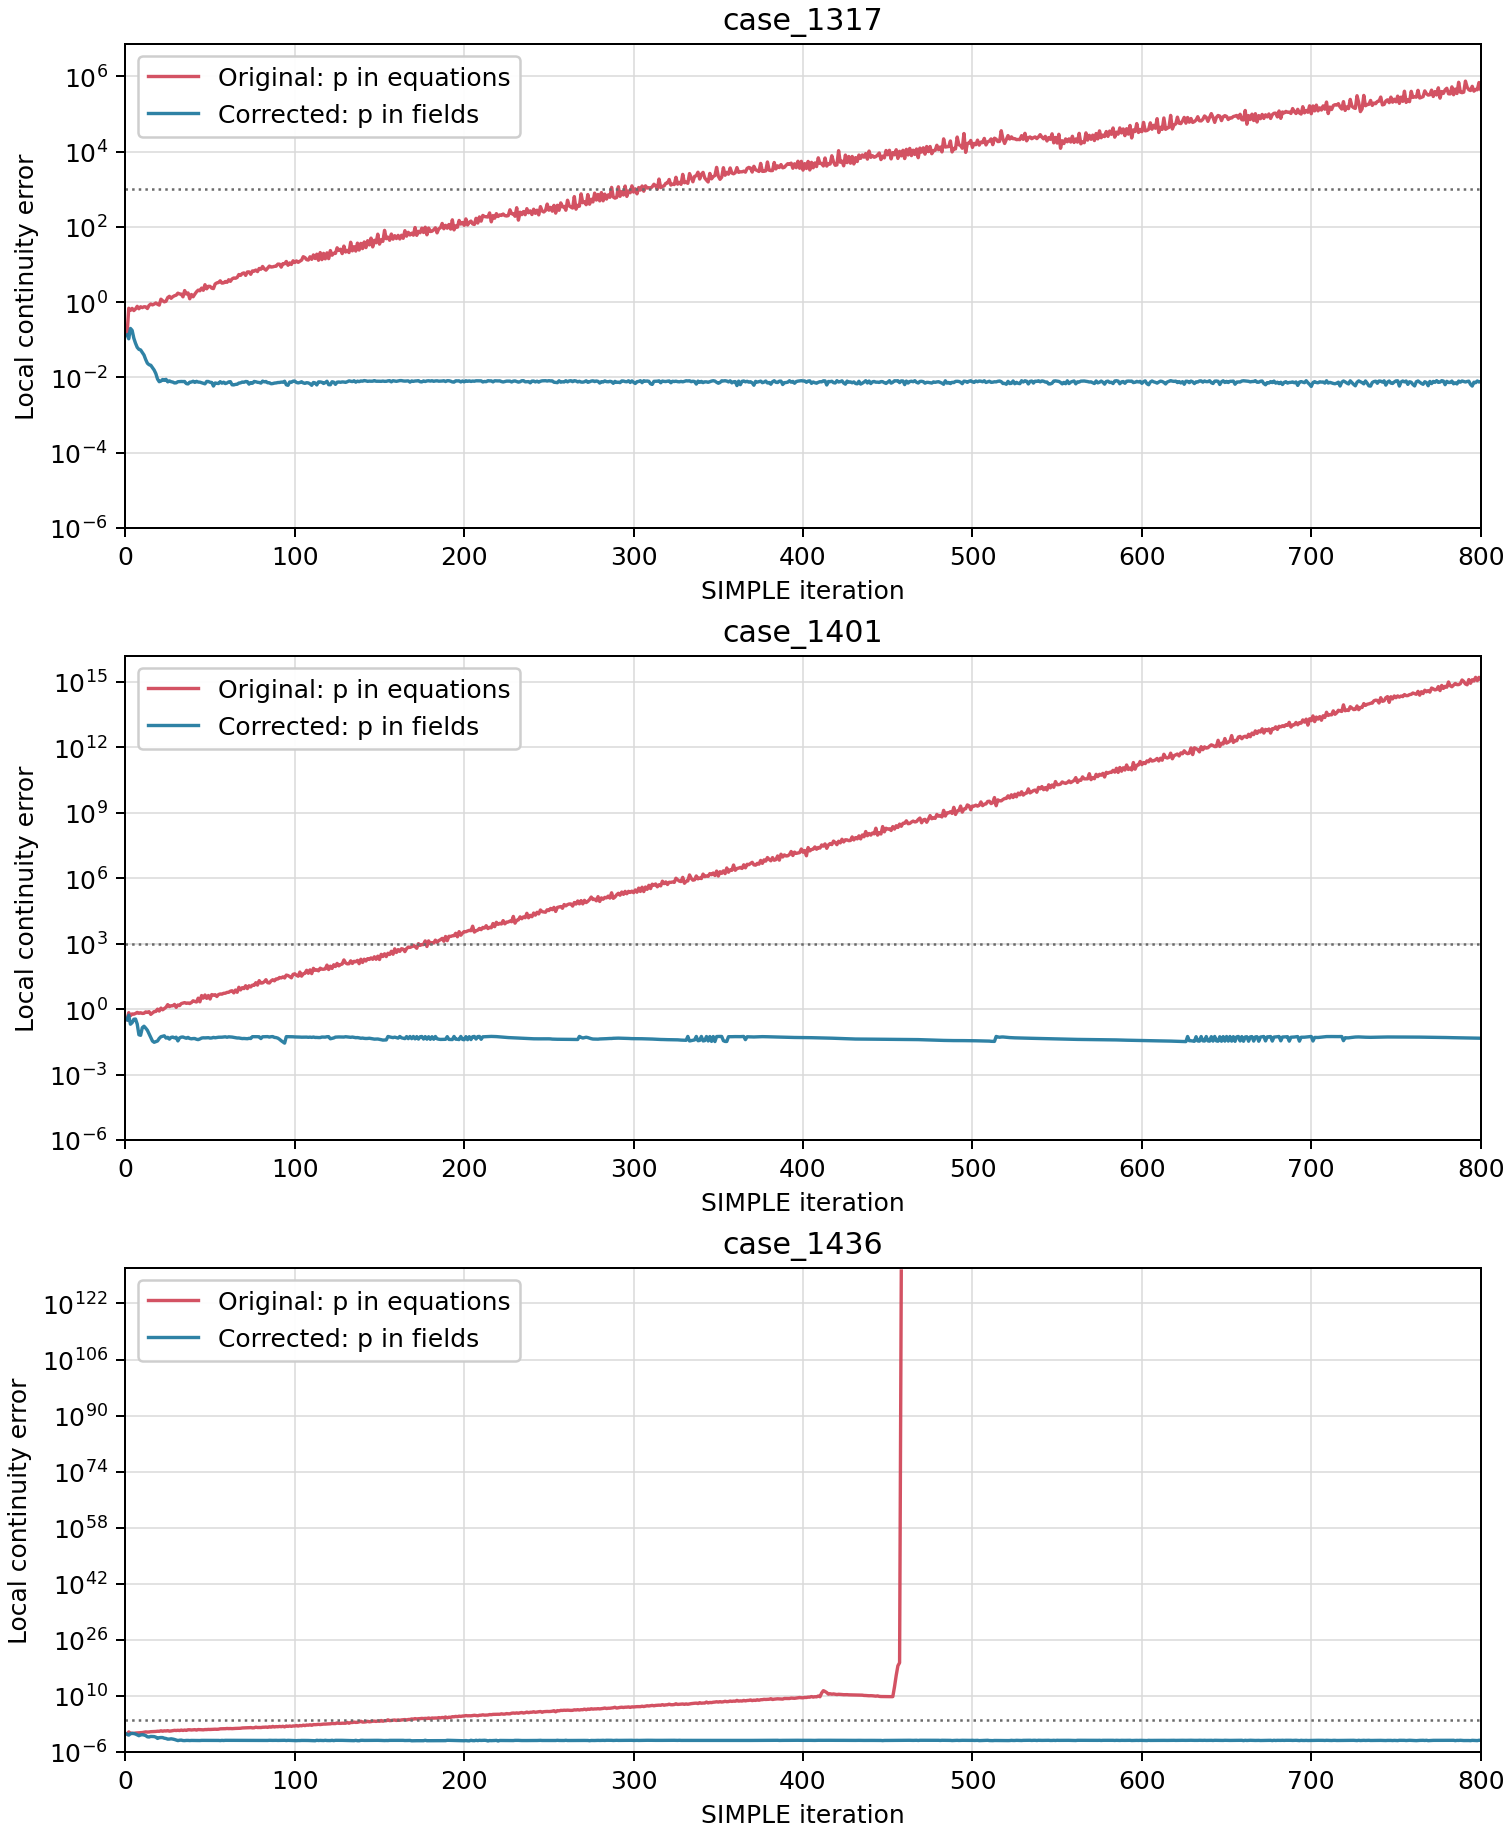
\includegraphics[width=\linewidth]{cfd_pressure_relaxation_ab_20260727.png}
  \caption{同一メッシュにおける修正前後のlocal continuity error。
  点線は$10^3$。青線は圧力をfield緩和へ移した最小修正である。}
\end{figure}

\subsection{別ケースでの再現}

\begin{center}
\begin{tabular}{lrrrl}
\toprule
ケース & 比較反復 & 元設定continuity & 修正後continuity & 修正後 \\
\midrule
\texttt{case\_1317} & 800 &
$4.57{\times}10^5$ & $7.87{\times}10^{-3}$ &
800完走、$U_{\max}=51.58$ m/s \\
\texttt{case\_1401} & 800 &
$1.27{\times}10^{15}$ & $4.61{\times}10^{-2}$ &
800完走、$U_{\max}=64.23$ m/s \\
\texttt{case\_1436} & 458 &
$1.82{\times}10^{131}$ & $2.21{\times}10^{-3}$ &
800完走、$U_{\max}=66.57$ m/s \\
\bottomrule
\end{tabular}
\end{center}

\texttt{case\_1436} は元設定では次の反復459でSIGFPEとなったが、
修正後は同じメッシュで800反復まで正常に進んだ。3形状で同じ結果が
得られたため、原因判定には再現性がある。

\subsection{本番ループ再開後の確認}

修正版テンプレートでディスパッチャを再開した。新規
\texttt{case\_1458} は
\[
 \theta_0=59.5338^\circ,\qquad L_1=5.1037~\mathrm{mm}
\]
であり、旧設定では観測27点中27点が失敗した高リスク領域内にある。
本番ジョブは反復960時点でlocal continuity error
$1.33\times10^{-3}$、それまでの最大値0.449であった。旧失敗群は
113--980反復でcontinuity errorが$10^3$を超えていたため、修正版の
本番ケースでも旧設定の初期発散が消えたことを確認した。これは完走前の
中間確認であり、最終場の有限性は従来の終了時速度検査でも判定する。

\section{適用した修正}

\texttt{base/system/fvSolution} を次の形へ変更した。

\begin{verbatim}
relaxationFactors
{
    fields
    {
        p               0.3;
    }

    equations
    {
        U               0.7;
        k               0.7;
        "(epsilon|omega)" 0.7;
    }
}
\end{verbatim}

\texttt{consistent yes}、一次風上のbounded div scheme、
\texttt{kOmegaSST} は変更していない。すなわち、A/B試験で必要性が
確認できた最小変更だけを本番テンプレートへ反映した。

\section{運用上の扱い}

\begin{enumerate}[leftmargin=24pt]
  \item 旧設定での \texttt{cfd\_failed} は物理的に不可能な設計点とは
    扱わない。目的GPの学習対象からは従来通り除外し、修正後設定で
    再評価可能とする。
  \item 高 \texttt{theta0\_deg} 領域を即座に幾何制約で削除しない。
    修正後の再計算結果に基づいて、物理的な制約が必要か判断する。
  \item \texttt{potentialFoam} の全件SIGFPEは2026年9月8日に修正済み。各hostの
    small batchで同じ正常終了を確認する。
  \item 実行時にcontinuity errorを監視し、明白な発散を早期停止する。
    現状は終了後の最大速度検査まで異常ケースが走ることがあり、
    計算時間を浪費する。
  \item \texttt{checkMesh} のdeterminant警告は成否を識別しなかったため、
    警告セルの位置を確認した上で別途メッシュ改善を行う。
\end{enumerate}

\section{再現用ファイル}

\begin{itemize}[leftmargin=24pt]
  \item 全ケース解析CSV：
    \texttt{reports/cfd\_failure\_cases\_20260727.csv}
  \item A/B試験要約：
    \texttt{reports/cfd\_pressure\_relaxation\_ab\_20260727.csv}
  \item 解析器：
    \texttt{tools/analyze\_cfd\_failures.py}
  \item 作図：
    \texttt{tools/plot\_cfd\_failure\_analysis.py}
  \item 診断ジョブ：
    \texttt{tools/run\_cfd\_diagnostic\_variant.sh}
\end{itemize}

\end{document}
